\chapter{定理证明工具\sctlprov{}}\label{chapt:sctlprov}
在上一章中,我们针对\SCTL{}证明系统设计了一种证明搜索策略并给出了证明搜索算法的伪代码。
在本章中,我们介绍对\SCTL{}的证明搜索算法的一个编程实现---定理证明工具\sctlprov{}(图\ref{workflow})以及该工具与其他模型检测工具的对比。
\sctlprov{}的工作方式如下:首先,\sctlprov{}读入一个输入文件,并将该输入文件解析到一个Kripke模型以及若干个\SCTL{}公式;然后,对于每个公式,\sctlprov{}搜索该公式的证明,如果该公式可证,则并输出该证明(或者只输出True),如果该公式不可证,则输出该公式的非的证明(或者只输出False)。

\begin{figure}[h]
	\centering
	\makebox[0.60\textwidth][c]{%
		\tiny
		\begin{tikzpicture}[
		outpt/.style={->,blue!80!black,very thick},
		outpt1/.style={->,red!80!black,very thick},
		>=stealth,
		every node/.append style={align=center}]
		
		\node [inputfile] (input) at (0,0) {
			\begin{tabular}{@{}c}
			\textsf{Input}\\\textsf{file}
			\end{tabular}};
		
		\node (preproc) at (1.5,0) {\textsf{Interpret}};
		
		\draw[outpt](input)--(preproc);
		
		\node (proofsearch) at (3.0,0) {
			\begin{tabular}{@{}l}
			\textsf{Proof}\\
			\textsf{search}
			\end{tabular}};
		
		\draw[outpt](preproc)--(proofsearch);
		
		\node [inputfile] (prooftree) at (7,1) {
			\begin{tabular}{@{}c}
			\textsf{Certificate} \\\textsf{or True}
			\end{tabular}};
		
		%\node (result) at (9, 0) {Provable/Unprovable};
		\node [inputfile] (result) at (7, -1) {
			\begin{tabular}{@{}c}
			\textsf{Counterexample} \\\textsf{or False}
			\end{tabular}};
		
		\node (sctlprov) at (2,0.5) {\sctl{}};
		\node (output) at (4.0,0.1) {\textsf{output}};
		\node (provable) at (5.3, 1.1) {\textsf{provable}};
		\node (unprovable) at (5.3,-1.15) {\textsf{unprovable}};
		
		%\node (output) at (6, 0.2) {output?};
		%\node (yes) at (6.85, 0.5) {yes};
		
		
		\begin{pgfonlayer}{background}
		\path (preproc.west |- sctlprov.north)+(-0.2,0.1) node (a) {};
		\path (proofsearch.east |- proofsearch.south)+(+0.2,-0.2) node (c) {};
		\path[fill=yellow!30,rounded corners, draw=black!50]
		(a) rectangle (c);
		\end{pgfonlayer}
		
		\begin{pgfonlayer}{background}
		\path (preproc.west |- preproc.north)+(-0.1,0.1) node (a) {};
		\path (preproc.east |- preproc.south)+(+0.1,-0.1) node (c) {};
		\path[fill=green!30,rounded corners, draw=black!50]
		(a) rectangle (c);
		\end{pgfonlayer}
		
		\begin{pgfonlayer}{background}
		\path (proofsearch.west |- proofsearch.north)+(-0.1,0.1) node (a) {};
		\path (proofsearch.east |- proofsearch.south)+(+0.1,-0.1) node (c) {};
		\path[fill=green!30,rounded corners, draw=black!50]
		(a) rectangle (c);
		\end{pgfonlayer}
		
		%\draw[blue!80!black,very thick, dashed](6.6, 0)--(6.6, 1);
		%\draw[blue!80!black,very thick](6.6, 1)--(prooftree);
		\draw[-,very thick, blue!80!black](3.55, 0)--(4.5, 0);
		\draw[-,very thick, blue!80!black](4.5, 0)--(4.5, 1);
		\draw[-,very thick, blue!80!black](4.5, 0)--(4.5, -1);
		\draw[outpt](4.5,-1)--(result);
		\draw[outpt](4.5,1)--(prooftree);
		\end{tikzpicture}}
	
	\caption{\sctl{}.}\label{workflow}
\end{figure}

\section{\sctlprov{}的输入语言}
本节讨论的是\sctlprov{}的输入语言。在\sctlprov{}中,输入语言的作用是定义\sctlprov{}的输入文件内容,即对计算机系统进行形式化建模,并定义要验证的性质,然后,\sctlprov{}可在该模型上验证该性质。

在绝大多数传统的\CTL{}模型检测工具的输入语言中,Kripke模型中的每个状态通常用固定个数的值来表示,其中值的类型通常相对较简单,比如布尔或枚举类型等。这类输入语言通常无法将状态表示为复杂的数据结构,比如任意有限长度的链表。在\sctlprov{}的输入语言中,我们可以利用多种类型的表达式来定义Kripke模型的状态,比如元组(tuple)、记录(record)、变体(variant)或者任意有限长度的链表等。当用这种表达式来表示状态时,状态之间的迁移则可用一个从状态映射到它的所有后继的函数来表示,而且原子公式(即状态的性质或者状态之间的关系)则可用一个从一个或者多个状态映射到一个布尔值的函数来表示。此类输入语言通常可以用来对复杂的系统进行建模,比如第\ref{subsc:sats}节中的小型飞机场运输系统。\sctlprov{}的输入语言的详细描述见附录\ref{chapt:sctl:input:language}。

\couic{In the input languages of most traditional model checkers, a state in a Kripke model is usually expressed as a bounded number of values, and the types of these value are rather simple, for instance, Booleans or enumerations of finite values, etc. Such kind of input languages usually cannot express states as complicated data structures such as lists with arbitrary finite length. In the input language of \sctlprov{}, we can define states as expressions of any types, for instance, tuples, records, variants, or lists with arbitrary finite length, etc. When expressing states in this way, transitions between states can be defined by any computable functions that mapping each state to a list of its successors, and atomic formulae (i.e., properties of a state or relations between states) can be defined as any computable functions that mapping a state, or a list of states into a Boolean value.
Such kinf of a input language can be used in the modeling of complex systems such as the Small Aircraft Transportation System in Section \ref{subsc:sats}. For further information about the input language of \sctlprov{}, the readers may refer to the documentations in the source code folder of the tool.}
%pre \textbf{\code{bold}} \code{face} 
%\begin{Verbatim}[commandchars=\\\{\},codes={\catcode`$=3\catcode`_=8}]
%\textbf{bold} face
%\end{Verbatim}
%post
\section{其他\CTL{}模型检测方法的对比}
在这里,我们讨论\sctlprov{}的证明搜索算法与其他\CTL{}模型检测方法的对比。

\paragraph{基于\BDD{}的符号模型检测}
当Kripke模型中绝大多数状态变量是布尔类型(比如在硬件模型检测问题中)的时候,\BDD{}的应用可以用来减少模型检测算法的空间占用。迄今为止,最好的基于\BDD{}的符号模型检测工具是\nusmv{}\cite{mcmillan93,CimattiCGR99}以及\nusmv{}的扩展\nuxmv{} \cite{CAVCDGMMMRT14}。下面我们举例说明基于\BDD{}的符号模型检测方法的原理:假设存在一个以$s_0$为初始状态,$T$为迁移规则的Kripke模型$\cal M$。若要验证${\cal M},s_0\models EF\phi$,基于\BDD{}的符号模型检测工具(例如\nusmv{})会首先计算一个最小不动点$\textup{lfp}=\mu Y. (\phi\vee EXY)$,然后,若$s_0\in \textup{lfp}$,则${\cal M},s_0\models EF\phi$成立,反之则不成立。计算不动点的过程中会不断地对迁移规则$T$进行展开直到得到不动点,其中$s_0$不可达的状态也可能被计算在不动点之内。

与基于\BDD{}的符号模型检测工具不同,\sctlprov{}在验证过程中没有必要计算不动点:迁移规则$T$是动态展开,即展开$T$直到可以判定公式是否可证为止。\sctlprov{}的验证过程只访问初始状态$s_0$可达的状态,因此验证过程会节省空间的占用。不止如此,当Kripke模型的状态变量绝大多数为布尔类型的时候,\sctlprov{}可以用\BDD{}来记录访问过的状态,并以此来进一步节省空间占用;反之,当Kripke模型中包含多个非布尔类型的状态变量的时候,\sctlprov{}可以选择直接记录(通常用哈希表)访问过的状态。不同于符号模型检测中将Kripke结构和要证明的性质都编码到\BDD{}的做法,\sctlprov{}在Kripke结构上直接做状态搜索,\BDD{}只被用来记录搜索过的状态。

\paragraph{即时(On-the-fly)模型检测}
在验证时序逻辑公式的正确性时,利用即时模型检测的方法可以避免访问Kripke模型的整个状态空间,而只是访问由初始状态可达的状态集合。传统的\CTL{}即时模型检测方法\cite{VergauwenL93,BCG95}通常是基于递归的:即子公式的验证以及迁移规则的展开都是递归进行的。基于递归的\CTL{}即时模型检测通常会涉及到大量的栈操作,尤其是在验证大型系统的过程中。验证算法通常会在栈操作上浪费大量的时间。

与传统的\CTL{}即时模型检测方法不同,在\sctlprov{}中,公式和迁移规则均按需展开,而且验证算法基于连续(连续传递风格)而不是递归。基于连续的算法只需占用常数大小的栈空间\cite{Reynolds93,Appel06,Sestoft12},而在递归算法中,栈空间的占用大小与递归深度成正比。

由于目前没有完整的基于传统的即时模型检测算法的工具存在,因此,为了将其与\sctlprov{}的证明搜索算法进行对比,我们开发了\sctlprov{}的一个递归版本,即\sctlprovr{}\footnote{\url{https://github.com/terminatorlxj/SCTLProV_R}}。不同于\sctlprov{},\sctlprovr{}利用基于递归的算法来证明子公式并搜索状态空间。\sctlprov{}与\sctlprovr{}的实验结果对比见第\ref{sec:case_exp}节。

\paragraph{限界模型检测}
在传统的限界模型检测工具中,若要证明一个时序逻辑公式,首先需要人为规定(或程序给定)一个限界,并将Kripke模型的迁移规则在限界之内展开,然后判断该公式在迁移规则的有限步展开之内满足与否。若在当前的限界之内可以判断公式满足与否,则算法终止;否则,继续扩大限界。举例来说,若要判断${\cal M}, s_0 \models_{k+1} EF\phi$满足与否,则要先在限界$k+1$之内展开公式与迁移规则\cite{BCCZ99}:

\begin{small}
	$$ [{\cal M},EF\phi]_{k+1} := \bigwedge^{k-1}_{i=0}T(s_i,s_{i+1}) \wedge \bigvee_{j=0}^k\phi(s_j)$$
\end{small}

与限界模型检测工具不同,\sctlprov{}不需要限界展开迁移规则,而是在展开证明公式的同时按需展开迁移规则。例如在证明$\vdash EF_x(\phi)(s_0)$的时候,公式和迁移规则的展开方式如下:

\begin{center}{\small
		$
		\textsf{unfold}(S,\vdash EF_x(\phi)(s_i)) := 
		\phi(s_i) \vee ((s_i\notin S) \wedge T(s_i, s_{i+1}) \wedge 
		\textsf{unfold}(S\cup \{s_i\},\vdash EF_x(\phi)(s_{i+1})))
		$
	}
\end{center}
其中,$S$是在证明过程中已经访问过的状态集合。




\section{案例分析}\label{sec:case_exp}

在本节中,我们讨论\sctlprov{}的两个应用案例:一个进程互斥问题和一个针对NASA提出的小型飞机场控制系统的形式化验证问题。


\subsection{案例一:进程互斥问题}\label{subsec:example}
\begin{example}[进程互斥问题\cite{Peterson81}]
	
	本例讲的是关于两个进程(进程$A$和进程$B$)的互斥问题。进程的互斥指的是在程序执行的任意时刻,最多只有一个进程在临界区内。一个关于此类问题的算法描述如图\ref{illustrative:mutual}所示,其中$flag$是一个布尔变量,指的是当前是否有进程在运行,而$mutex$是一个整型变量,指的是当前进入临界区的进程个数(初始值为$0$)。如果在程序执行的某个时刻有多于$1$个进程进入临界区(即$mutex=2$),那么则称该程序违反了进程互斥性质。
	
	\begin{figure}[h!]
		\centering
		\small
		\begin{tabular}{p{5.3cm}p{3.8cm}}
			\begin{verbatim}
			/* Process A */
			1: while(flag);/*wait*/
			2: flag = true;
			3: mutex ++;
			/*critical section*/
			4: mutex --;
			5: flag = false;
			\end{verbatim}
			&
			\begin{verbatim}
			/* Process B */
			1: while(flag);/*wait*/
			2: flag = true;
			3: mutex ++;
			/*critical section*/
			4: mutex --;
			5: flag = false;
			\end{verbatim}
		\end{tabular}
		\label{illustrative:mutual}
		\caption{进程$A$和进程$B$的一个简单描述。}
	\end{figure}
	
	\begin{figure}[!h]
		\centering
		\scriptsize
		%		\framebox{
		\begin{boxedverbatim}
			Model mutual()
			{
				Var {
					flag : Bool; mutex : (0 .. 2); a : (1 .. 5); b : (1 .. 5);
				}
				Init {
					flag := false; mutex := 0; a := 1; b := 1;
				}
				Transition {
					a = 1 && flag = false : {a := 2;};
					a = 2 : {a := 3; flag := true;};
					a = 3 : {a := 4; mutex := mutex + 1;}; /*A has entered the critical section*/
					a = 4 : {a := 5; mutex := mutex - 1;}; /*A has left the critical section*/ 
					a = 5 : {flag := 0;};
					b = 1 && flag = false : {b := 2;};
					b = 2 : {b := 3; flag := true;};
					b = 3 : {b := 4; mutex := mutex + 1;}; /*B has entered the critical section*/
					b = 4 : {b := 5; mutex := mutex - 1;}; /*B has left the critical section*/ 
					b = 5 : {flag := 0;};
					/*If none of the conditions above are satisfied, then the current state goes to itself.*/
					(a = 1 || b = 1) && flag = true: {}
				}
				Atomic {
					bug(s) := s(mutex = 2);
				}
				Spec {
					find_bug := EU(x, y, TRUE, bug(y), ini);
				}
			}
		\end{boxedverbatim}
		%	}
		\caption{输入文件“mutual.model”。}
		\label{fig:mutual}
	\end{figure}
	如图\ref{fig:mutual}所示,输入文件"mutual.model"中变量$a$和变量$b$分别指代进程$A$和进程$B$的程序计数器(Program Counter),变量$ini$指代初始状态。本例中要验证的性质为:是否存在程序执行的某个时刻使得两个进程同时进入临界区。利用\sctlprov{},我们可以在计算机的命令行中输入以下命令来验证该性质。
	\begin{center}
		\small
		\begin{verbatim}
		sctl -output output.out mutual.model
		\end{verbatim}
	\end{center}
	
	%	The result is as follows, which indicates that there is a bug in the mutual exclusion problem, i.e., the mutual exclusion property is violated.
	\sctlprov{}的运行结果如下所示:该程序存在漏洞,即该程序违反了进程互斥性质。
	\begin{center}
		\small
		\begin{verbatim}
		verifying on the model mutual...
		find_bug: EU(x,y, TRUE, bug(y), ini)
		find_bug is true.
		\end{verbatim}
	\end{center}
	该性质的证明树输出在文件"output.out"中,如下图所示。证明树的每个节点被输出为${id: seqt ~ [id_1, ..., id_n]}$形式,其中$id$是该节点的ID,$seqt$是当前的相继式,而${id_1,...,id_n}$则是当前的相继式的所有的前提的ID。
	\begin{center}
		\small
		\begin{verbatim}
		0: |- EU(x,y,TRUE,bug(y),{flag:=false;mutex:=0;a:=1;b:=1})	[4, 1]
		4: {flag:=false;mutex:=0;a:=1;b:=1}
		|- EU(x,y,TRUE,bug(y),{flag:=false;mutex:=0;a:=2;b:=1})	[7, 5]
		1: |- TRUE	[]
		7: {flag:=false;mutex:=0;a:=1;b:=1} 
		{flag:=false;mutex:=0;a:=2;b:=1}
		|- EU(x,y,TRUE,bug(y),{flag:=false;mutex:=0;a:=2;b:=2})	[23, 20]
		5: |- TRUE	[]
		23:{flag:=false;mutex:=0;a:=1;b:=1} 
		{flag:=false;mutex:=0;a:=2;b:=1} 
		{flag:=false;mutex:=0;a:=2;b:=2}
		|- EU(x,y,TRUE,bug(y),{flag:=true;mutex:=0;a:=3;b:=2})	[27, 24]
		20: |- TRUE	[]
		27:{flag:=false;mutex:=0;a:=1;b:=1} 
		{flag:=false;mutex:=0;a:=2;b:=1} 
		{flag:=false;mutex:=0;a:=2;b:=2} 
		{flag:=true;mutex:=0;a:=3;b:=2}
		|- EU(x,y,TRUE,bug(y),{flag:=true;mutex:=1;a:=4;b:=2})	[31, 28]
		24: |- TRUE	[]
		31:{flag:=false;mutex:=0;a:=1;b:=1} 
		{flag:=false;mutex:=0;a:=2;b:=1} 
		{flag:=false;mutex:=0;a:=2;b:=2} 
		{flag:=true;mutex:=0;a:=3;b:=2} 
		{flag:=true;mutex:=1;a:=4;b:=2}
		|- EU(x,y,TRUE,bug(y),{flag:=true;mutex:=1;a:=4;b:=3})	[35, 32]
		28: |- TRUE	[]
		35:{flag:=false;mutex:=0;a:=1;b:=1} 
		{flag:=false;mutex:=0;a:=2;b:=1} 
		{flag:=false;mutex:=0;a:=2;b:=2} 
		{flag:=true;mutex:=0;a:=3;b:=2} 
		{flag:=true;mutex:=1;a:=4;b:=2} 
		{flag:=true;mutex:=1;a:=4;b:=3}
		|- EU(x,y,TRUE,bug(y),{flag:=true;mutex:=2;a:=4;b:=4})	[37]
		32: |- TRUE	[]
		37: |- bug({flag:=true;mutex:=2;a:=4;b:=4})	[]
		\end{verbatim}
	\end{center}
	由以上的证明树输出可知,当进程$A$进入临界区之后,进程$B$同样进入临界区。
	
	如图\ref{fig:visualize:illustrative}所示,\sctlprov{}验证该例子时的输出(证明树和Kripke模型)可由可视化工具\tool{VMDV}(Visualization for Modeling, Demonstration, and Verification)实现三维可视化显示。
	\begin{figure}[!h]
		\centering
		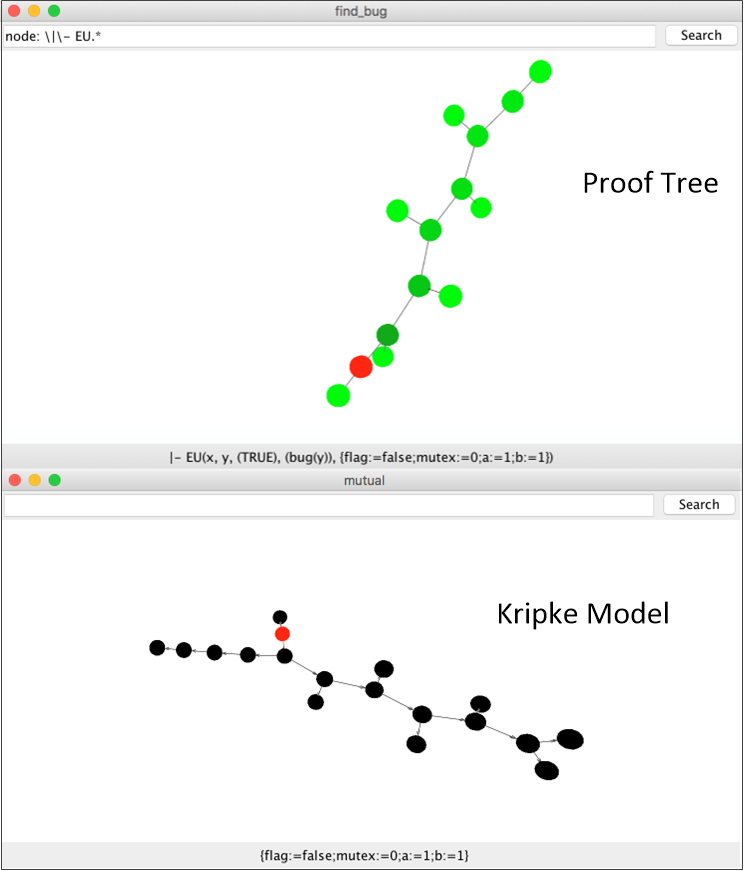
\includegraphics[width=10cm]{./illustrative_example2.png}
		\caption{进程互斥问题的验证中证明树和模型的可视化}
		%		\caption{Visualization of the proof tree and the Kripke model in the illustrative example.}
		\label{fig:visualize:illustrative}
	\end{figure}
	
	通过对原程序进行修改\cite{Peterson81},可以使程序满足进程互斥性质,修改后的程序如图\ref{illustrative:mutual:solution}所示。修改后的程序可形式化描述为图\ref{fig:mutual:solution}所示的输入文件。在此输入文件中,变量$x$和变量$y$均为布尔变量,分别指代当前状态下进程$A$和进程$B$是否在运行,而$turn$则表示进程$A$和进程$B$轮流处在临界区内。
	
	\begin{figure}[!h]
		\centering
		\small
		\begin{tabular}{p{5.8cm}p{4.8cm}}
			\begin{verbatim}
			/* Process A */
			1: x = true;
			2: turn = 1;
			3: while(y&&turn!=2); /*wait*/
			4: mutex ++;
			/*critical section*/
			5: mutex --;
			6: x = false;
			\end{verbatim}
			&
			\begin{verbatim}
			/* Process B */
			1: y = true;
			2: turn = 2;
			3: while(x&&turn!=1); /*wait*/
			4: mutex ++;
			/*critical section*/
			5: mutex --;
			6: y = false;
			\end{verbatim}
		\end{tabular}
		
		\caption{修改后的进程互斥程序}
		\label{illustrative:mutual:solution}	
	\end{figure}
	
	\begin{figure}[h!]
		\centering
		\scriptsize
		%		\begin{tabular}{|c|}
		
		%		\begin{minipage}{10cm}
		\begin{boxedverbatim}
			Model mutual()
			{
				Var {
					x:Bool; y:Bool; mutex:(0 .. 2); turn:(1 .. 2); a:(1 .. 6); b:(1 .. 6);
				}
				Init {
					x := false; y := false; mutex := 0; turn := 1; a := 1; b := 1;
				}	
				Transition {
					a = 1 : {a := 2; x := true;};
					a = 2 : {a := 3; turn := 1;};
					a = 3 && (y = false || turn = 2): {a := 4;}; 
					/*A has entered the critical section*/
					a = 4 : {a := 5; mutex := mutex + 1;}; 
					/*A has left the critical section*/
					a = 5 : {a := 6; mutex := mutex - 1;}; 
					a = 6 : {x := false;};
					b = 1 : {b := 2; y := true;};
					b = 2 : {b := 3; turn := 2;};
					b = 3 && (x = false || turn = 1): {b := 4;}; 
					/*B has entered the critical section*/
					b = 4 : {b := 5; mutex := mutex + 1;}; 
					/*B has left the critical section*/
					b = 5 : {b := 6; mutex := mutex - 1;}; 
					b = 6 : {y := false;};
					/*If none of the conditions above are satisfied, 
					then the current state goes to itself.*/
					(a != 3 && (y = true && turn = 1)) || (b != 3 && (x = true && turn = 2)) : {};
				}
				Atomic {
					bug(s) := s(mutex = 2);
				}
				Spec {
					find_bug := EU(x, y, TRUE, bug(y), ini);
				}
			}
			
		\end{boxedverbatim}
		%	\end{minipage}
		%	\end{tabular}
		\caption{输入文件“mutual\_solution.model”}
		\label{fig:mutual:solution}
	\end{figure}
	
	%	The verification result of this model would be as follows.
	%	When applying this solution, the mutual exclusion exclusion property will not be violated, which is indicated by the following result.
	如下所示,修改后的程序满足进程互斥性质。
	\begin{center}
		\small
		\begin{verbatim}
		verifying on the model mutual...
		find_bug: EU(x, y, TRUE, bug(y), ini)
		find_bug is false.
		\end{verbatim}
	\end{center}
\end{example}

\subsection{案例二:小型飞机场运输系统}\label{subsc:sats}
在本小节中,我们介绍对于一个工程问题的形式化验证:由美国国家航空与航天局(National Aeronautics and Space Administration,简称NASA)为主导提出的小型飞机场运输系统(Small Aircraft Transportation System,简称SATS)\cite{MunozDC04,nasasats04}。在\sctlprov{}中,我们对SATS系统进行形式化描述,并验证该系统的安全性。



\begin{figure}
	\centering
	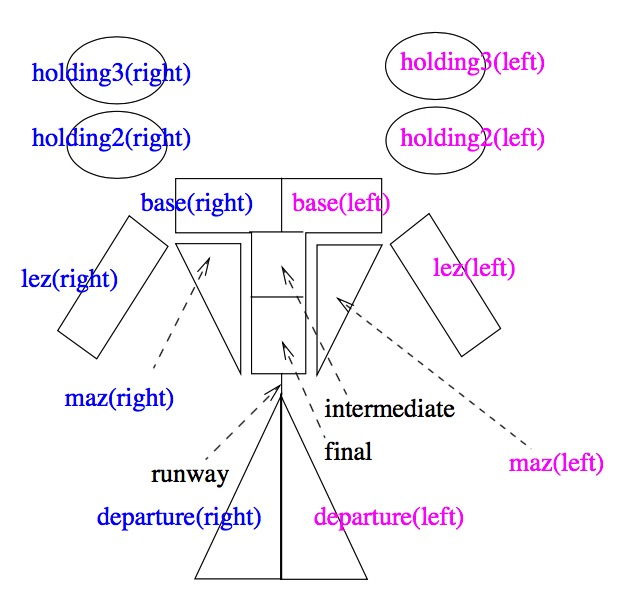
\includegraphics[width=9cm]{./sca.jpg}
	\caption{飞机场自我控制区域的划分(以飞行员视角区分左右)}
	%	\caption{SCA zones, where right and left are relative to the pilot facing the runway, i.e., opposite from the reader point of view \cite{MunozDC04}.}
	\label{fig:example:sats:sca}
\end{figure}

在SATS系统中,整个飞机场区域被称为自我控制区(Self Control Area,简称SCA)。如图\ref{fig:example:sats:sca}所示,该模型将SCA被分为15个子区域:
\begin{itemize}
	\item \textbf{holding3(right/left)}:等待航线,高度3000英尺(右/左);
	\item \textbf{holding2(right/left)}:等待航线,高度2000英尺(右/左);
	\item \textbf{lez(right/left)}:水平降落航线(右/左);
	\item \textbf{base(right/left)}:基地航线(右/左);
	\item \textbf{intermediate}:中间航线;
	\item \textbf{final}:最终航线;
	\item \textbf{runway}:机场跑道;
	\item \textbf{maz(right/left)}:重新降落航线(右/左);
	\item \textbf{departure(right/left)}:起飞航线(右/左)。
\end{itemize}
在任意时刻,SCA的每个子区域内都有若干架飞机,每个子区域内的飞机遵循先进先出的顺序依次进出。在整个SCA中,飞机的进出子区域的方式有24种,分别如下:
\begin{itemize}
	\item 进入3000英尺高度等待航线(右/左);
	\item 进入水平降落航线(右/左);
	\item 从3000英尺等待航线进入2000英尺等待航线(右/左);
	\item 从2000英尺等待航线进入基地航线(右/左);
	\item 从水平降落航线进入基地航线(右/左);
	\item 从基地航线(右/左)进入中间航线;
	\item 从中间航线进入重新降落航线(右/左);
	\item 从中间航线进入最终航线;
	\item 准备降落,从最终航线进入机场跑道;
	\item 降落成功,飞机驶离机场跑道;
	\item 降落失败,从最终航线进入重新降落航线(右/左);
	\item 从重新降落航线进入高度最低,而且可以进入(当前等待航线中没有飞机)的等待航线;
	\item 进入机场跑道并准备起飞;
	\item 从机场跑道进入起飞航线;
	\item 从起飞航线(右/左)离开,最终离开SCA。
\end{itemize}
在任意时刻,飞机进出SCA的子区域的方式必须是安全的,即SATS系统必须满足8个性质:
\begin{itemize}
	\item SCA中不超过4架飞机同时准备降落:即等待航线,水平降落航线,重新降落航线,基地航线,中间航线,以及最终航线上飞机的总数不超过4;
	\item SCA中左右两侧的航线(等待航线,水平降落航线,以及重新降落航线)中,同侧的飞机数总和不超过2,同时SCA中不超过2架飞机准备从同侧重新降落航线重新降落;
	\item 进入SCA的航线(等待航线和水平进入航线)中,每个航线每侧的飞机数不超过2,同时基地航线的飞机数总和不超过3;
	\item 在每侧的水平进入航线中最多只有一架飞机,同时如果某侧水平进入航线中有飞机,则SCA的同侧其他航线(水平降落航线以及重新降落航线)中没有飞机;
	\item SCA中的飞机按照事先给定的顺序依次进入SCA;
	\item 最先进入SCA中飞机一定最先降落;
	\item 机场跑道上最多只有一架飞机;
	\item 起飞航线上的飞机彼此必须相隔足够远的距离。
\end{itemize}
在\sctlprov{}中,我们针对SCA建立一个Kripke模型:模型中的状态用15个状态变量来表示,分别代表SCA中15个子区域,每个状态变量都是列表类型,代表该子区域内的若干架飞机;模型中包含24条迁移规则,分别指代SCA中的所有飞机在每个子区域间的24种进出方式;要验证的性质是一个\ctlpm{}公式,即在每个状态上,SCA都满足安全性质。该模型的输入文件可在因特网\footnote{\url{https://github.com/sctlprov/sctlprov_sats}}上下载。

\sctlprov{}验证该模型用时26秒左右,运行环境为:Linux操作系统,内存3.0GB,2.93GHz$\times$4 CPU。验证过程中共访问54221个状态(Dowek,Mu\~noz和Carre\~no提出了对SATS系统的一个简化版的PVS建模\cite{MunozDC04},在该模型中可访问的状态数为2811)。
经\sctlprov{}验证,该模型满足安全性性质。


\couic{The model is
	non-deterministic, that is, for a given state, several transitions are
	possible and all must be considered.  As there are no a
	priori bounds on the number of aircraft in each zone, the number of
	states in the model is potentially infinite. However, the number of
	states that are reachable from the initial state is finite: 
	an enumeration of the model shows that there are 54221 such states (and
	around 3000 in the simplified model where departure operations are not
	considered).
	
	There are eight properties of the model that we want to 
	verify with \sctl{}, for instance that 
	the \textsf{SATS} concept does not allow more than four simultaneous 
	landing operations and none of the 
	15 zones contains too many aircraft (each zone is
	assigned a maximum number of aircraft and the actual number of
	aircraft is never higher than this number).
	The safety property is thus conjunction of these eight properties. 
	
	The verification problem is to check that this
	property holds on every reachable state from the initial state (the
	state where there are no aircraft on each zone of the self controlled
	area), so the formula to be checked is $AG_x(\phi)(e)$ where $\phi$ is 
	the conjunction of the eight properties and $e$ is the initial state.
}

值得注意的是,虽然这是一个典型的模型检测问题,但是传统的模型检测工具均无法验证该模型\cite{MunozDC04},理由如下:
\couic{This is a typical model checking problem, but this problem
	is known to be cumbersome for traditional model checkers
	\cite{MunozDC04} because:}
\begin{enumerate}
	\couic{\item Each state of the model is represented by a complex data
		structure. For instance, a number of state variables are
		represented by lists of aircraft with unbounded length.}
	\item 模型的状态由复杂的数据结构所表示:每个状态变量的值均为列表类型,而且列表的长度可能为无穷。
	\couic{\item The transition rules of the model are 
		complex algorithms. For instance, some transitions rules
		involve recursive operations on lists of aircraft.}
	\item 状态的迁移规则必须由复杂的算法所描述:在某些状态迁移的过程中需要对飞机列表进行递归操作。
	\couic{\item The
		properties to be verified in the model are also represented
		by complex algorithms. For instance, some of the properties
		are inductively defined over lists of aircraft.}
	\item 模型的性质必须由复杂的算法所描述:某些原子命题的定义需要对飞机列表进行递归操作。
\end{enumerate}
\sctlprov{}的输入语言表达能力强于绝大多数模型检测工具,并能完整的表示该模型,同时成功进行验证。

\couic{However, this example fits well in \sctl{} that provides a
	more expressive input language than most traditional model
	checkers. Indeed, \sctl{} provides both readable notations for the
	definition of data structures such as records or lists with unbounded
	length, and arbitrary algorithms for the definitions of transition
	rules and of properties.  So we have been able to check in
	\sctl{} that the safety property holds on the model, and the
	verification was executed in less than 30 seconds on the same machine as which the benchmarks are evaluated.}
\section{与相关工具的实验结果对比}
在本节中,我们分别对比\sctlprov{}和其他5个工具在4个测试集上的实验结果。
被用于与\sctlprov{}对比的5个工具分别为:基于\BDD{}的符号模型检测工具\nusmv{}及\nuxmv,基于\QBF{}的限界模型检测工具\verds{},基于消解(Resolution)的定理证明工具\tool{iProver Modulo},以及形式验证工具包\CADP{}。
本节所有工具的运行环境均为:Linux操作系统,内存3.0GB,2.93GHz$\times$4 CPU;每个测试用例的最大运行时间限制为20分钟。本节所有的测试用例均可在因特网\footnote{\url{https://github.com/sctlprov/sctlprov_benchmarks}}下载。
\subsection{随机生成的布尔程序的验证}\label{subsec:random}
本小节包含两个测试集:测试用例集一在首次提出\cite{Zhang14}时被用作对比限界模型检测工具\verds{}和符号模型检测工具\nusmv{}的性能;并紧接着被用作对比定理证明器\tool{iProver Modulo}与\verds{}的性能;在测试集一的基础上,我们通过增大模型中的状态变量的个数而得到测试集二。测试集一中包含2880个测试用例,测试集二中包含5760个测试用例。测试集一、二中的每个测试用例的Kripke模型都是随机生成的,每个模型中的状态变量绝大多数为布尔类型。大量的随机的测试用例对于\sctlprov{}与不同的工具来说都是相对公平的,而且通过对比不同工具的实验结果数据,我们可以清晰的得出有关各个工具在验证不同的模型以及不同的性质时的优势与劣势的结论。

以下分别介绍这两个测试集。

\couic{We consider three benchmarks in this part. 
	The original description of benchmark \#1 \cite{Zhang14} is restated here.
	Based on benchmark \#1, we extend the number of variables to tens, hundreds, and even thousands in benchmark \#2 and benchmark \#3.
	The randomness of the test cases in three benchmarks makes it rather fair for different \CTL{} model checking approaches, and helps us recognize the strengths and weaknesses of each tool. }

\subsubsection{测试集一}
\couic{Benchmark \#1 chosen in this subsection is originally introduced by Zhang \cite{Zhang14} in the evaluation of model checkers \verds{} and \nusmv{}. Later, Ji \cite{Ji15} also uses this benchmark in the evaluation of the theorem prover \tool{iProver Modulo} and the model checker \verds{}. This benchmark consists of 2880 randomly generated test cases where two types of random Boolean programs are considered---Concurrent Processes and Concurrent Sequential Processes. 
	In programs with Concurrent Processes,
	the parameters of the first set of random Boolean programs are as
	follows.}

测试集一中包含两类测试用例:并发进程(Concurrent Processes,简称CP)和并发顺序进程(Concurrent Sequential Processes,简称CSP)。
\paragraph{并发进程}
在描述并发进程需要用到以下4个变量:

\begin{center}
	\begin{tabular}{|l|}
		\hline
		$a$: 进程个数 \\
		$b$: 所有进程的共享变量和局部变量的个数 \\
		$c$: 进程间共享变量的个数 \\
		$d$: 每个进程的局部变量的个数 \\
		\hline
	\end{tabular}
\end{center}
进程间的共享变量的初始值均为$\{0,1\}$中的随机值,而每个进程的局部变量的初始值均为$0$。每个进程的共享变量和局部变量的每次赋值均为随机选择的某个变量的值的逻辑非。我们令每个测试用例中进程个数为3,即$a=3$;令$b$在$\{12,24,36\}$中取值;同时令$c=b/2$,以及$d=c/a$。对于每个$b$的取值有20个Kripke模型,然后在每个Kripke模型分别验证24个\CTL{}性质。因此,此测试集中共有$3\times20\times24=1440$个并发进程测试用例。

\couic{The shared variables are initially set to a random value in $\{0,1\}$,
	and the local variables are initially set to $0$. For each process,
	the shared variables and the local variables are assigned the negation
	of a variable randomly chosen from these variables. We test different
	sizes of the programs with 3 processes ($a=3$), and let $b$ vary over
	the set of values $\{12,24,36\}$, then set $c=b/2, d=c/a$. Each of the
	24 properties is tested on 20 test cases for each value of $b$.}

\paragraph{并发顺序进程} 
在并发顺序进程测试用例中,除了以上定义的$a,b,c,d$变量之外,描述该类型测试用例还需用到以2个变量:

\couic{In programs with Concurrent Sequential Processes,
	in addition to $a,b,c,d$ specified above, the parameters of the second set of random Boolean programs are as
	follows.}
\begin{center}
	\begin{tabular}{|l|}
		\hline
		$t$: 每个进程的迁移的个数 \\
		$p$: 在每个迁移过程中同时进行的赋值的个数\\
		\hline
	\end{tabular}
\end{center}
除了在并发进程中介绍的$b$个布尔变量之外,在每个并发顺序进程中还用到一个局部变量来表示进程当前执行的位置,共有$c$个取值。进程间的共享变量的初始值均为$\{0,1\}$中的随机值,而每个进程的局部变量的初始值均为$0$。每个进程共有$t$种迁移(状态变换,即对变量的赋值操作),在每个迁移种对随机选择的$p$个共享变量和局部变量进行赋值操作。随着进程的运行,所有的迁移依次周期性地进行。我们令每个测试用例包含2个进程,即$a=2$;令$b$在$\{12,16,20\}$中取值;同时令$c=b/2,d=c/a,t=c,p=4$。对于每个$b$的取值有20个Kripke模型,然后在每个Kripke模型分别验证24个\CTL{}性质。因此,此测试集中共有$3\times20\times24=1440$个并发顺序进程测试用例。
\couic{For each concurrent sequential process, besides the $b$ Boolean
	variables, there is a local variable representing program locations,
	with $c$ possible values. The shared variables are initially set to a
	random value in $\{0,1\}$, and the local variables are initially set
	to $0$. For each transition of a process, $p$ pairs of shared
	variables and local variables are randomly chosen among the shared
	variables and the local variables, such that the first element of such
	a pair is assigned the negation of the second element of the
	pair. Transitions are numbered from $0$ to $t-1$, and are executed
	consecutively, and when the end of the sequence of the transitions is
	reached, it loops back to the execution of the transition numbered
	$0$. For this type of programs, we test different sizes of the
	programs with $2$ processes ($a=2$), and let $b$ vary in the set of
	values $\{12,16,20\}$, and then set $c=b/2, d=c/a, t=c$, and
	$p=4$. Similarly, each property is tested on $20$ test cases for each
	value of $b$.}

在本测试集中,我们验证24个\CTL{}性质,其中性质$P_{01}$至 $P_{12}$如图\ref{fig:properties}所示,而性质$P_{13}$至$P_{24}$为依次将$P_{01}$至 $P_{12}$中的$\wedge$替换成$\vee$,以及将$\vee$替换成$\wedge$。

\couic{Twenty-four properties are to be checked in this benchmark: properties $P_{01}$ to $P_{12}$ are depicted in Figure~\ref{fig:properties}, and $P_{13}$ to $P_{24}$ are simply the variations of
	$P_{01}$ to $P_{12}$ by replacing $\wedge$ and $\bigvee$ by $\vee$ and
	$\bigwedge$, respectively.}

\begin{figure}[!h]
	\centering
	{
		\begin{tabular}{|l|l||l|l|}
			\hline
			$P_{01}$& $AG(\bigvee^c_{i=1}v_i)$ & $P_{07}$& $AU(v_1, AU(v_2, \bigvee^c_{i=3}v_i))$\\
			\hline
			$P_{02}$& $AF(\bigvee^c_{i=1}v_i)$ & $P_{08}$ & $AU(v_1, EU(v_2, \bigvee^c_{i=3}v_i))$\\
			\hline
			$P_{03}$& $AG(v_1 \A AF(v_2\wedge \bigvee^c_{i=3}v_i))$ & $P_{09}$& $AU(v_1, AR(v_2, \bigvee^c_{i=3}v_i))$\\
			
			\hline
			$P_{04}$& $AG(v_1 \A EF(v_2\wedge \bigvee^c_{i=3}v_i))$ & $P_{10}$& $AU(v_1, ER(v_2, \bigvee^c_{i=3}v_i))$\\
			
			\hline
			$P_{05}$& $EG(v_1 \A AF(v_2\wedge \bigvee^c_{i=3}v_i))$ & $P_{11}$& $AR(AX v_1, AX AU(v_2, \bigvee^c_{i=3}v_i))$\\
			
			\hline
			$P_{06}$& $EG(v_1 \A EF(v_2\wedge \bigvee^c_{i=3}v_i))$ & $P_{12}$& $AR(EX v_1, EX EU(v_2, \bigvee^c_{i=3}v_i))$\\
			
			\hline
		\end{tabular}
	}
	\caption{测试集一中需要验证的性质$P_{01}$至$P_{12}$}
	\label{fig:properties}
\end{figure}

\subsubsection{测试集二}
在测试集一的基础上,我们分别将并发进程测试用例中$b$的值分别扩大为$48$、$60$、$72$、$252$、$504$、$1008$,将并发顺序进程测试用例中$b$的值分别扩大为$24$、$28$、$32$、$252$、$504$、$1008$。由此,我们得到包含5760个新的测试用例的测试集二。与测试集一一样,测试集二中的测试用例的模型的初始状态和迁移规则也是随机生成的。测试集二中要验证的性质与测试集一一致。

%在测试集三中,我们将并发进程和并发顺序进程测试用例的$b$的值同时进一步扩大到$252$,$504$,以及$1008$,同时要验证的性质与测试集一、二保持一致。

\subsubsection{实验数据}
\couic{The experimental results are shown below, and the detailed data is in \ref{app:detail:data}.}
在测试集一、二上,我们分别对比了\sctlprov{}与\tool{iProver Modulo}、\verds{}、\nusmv{},以及\nuxmv{}的实验结果。

\paragraph{测试集一的实验结果}
由表\ref{tabl:solvable}与表\ref{tabl:compare}可知:在测试集一的2880个测试用例中,\tool{iProver Modulo}、\verds{}、\nusmv{}、\nuxmv{}、\sctlprov{}分别能验证1816(63.1\%)、2230(77.4\%)、2880(100\%)、2880(100\%)、2862(99.4\%)个测试用例;同时\sctlprov{}分别在2823(98.2\%)、2858(99.2\%)、2741(95.2\%)、2763(95.9\%)个测试用例上占用时间和空间少于\tool{iProver Modulo}、\verds{}、\nusmv{}、\nuxmv{}。各个工具的时间占用随着状态变量的个数的变化趋势如图\ref{fig:average_time:extended}所示;各个工具占用空间随着状态变量的个数的变化趋势如图\ref{fig:average_memory:extended}所示。


\begin{table}[!h]\small
	%	\begin{tabular}{c c}
	%\renewcommand{\arraystretch}{1.0}
	%		\begin{minipage}[b]{0.5\linewidth}
	\centering
	\setlength{\tabcolsep}{1pt}
	\begin{tabular}{| l | r | r | r | r | r |}
		\hline
		\textbf{程序类型} & \tool{iProver Modulo} & \verds{} & \nusmv{} & \nuxmv{} & \sctl{}\\
		\hline
		\code{CP ($b = 12$)} & 467(97.3\%) & 433(90.2\%) & 480(100\%) & 480(100\%) & 480(100\%)\\
		\hline
		
		%\hline
		\code{CP ($b = 24$)} & 372(77.5\%) & 428(89.2\%) & 480(100\%) & 480(100\%) & 480(100\%)\\
		\hline
		
		%\hline
		\code{CP ($b = 36$)} & 383(79.8\%) & 416(86.7\%) & 480(100\%) & 480(100\%) & 470(97.9\%)\\
		\hline
		
		%\hline
		\code{CSP ($b = 12$)} & 177(36.9\%) & 370(77.1\%) & 480(100\%) & 480(100\%) & 480(100\%)\\
		\hline
		
		%\hline
		\code{CSP ($b = 16$)} & 164(34.2\%) & 315(65.6\%) & 480(100\%) & 480(100\%) & 474(98.8\%)\\
		\hline
		
		%\hline
		\code{CSP ($b = 20$)} & 253(52.7\%) & 268(55.8\%) & 480(100\%) & 480(100\%) & 478(99.6\%)\\
		\hline
		Sum & 1816(63.1\%) & 2230(77.4\%) & 2880(100\%) & 2880(100\%) & 2862(99.4\%)\\
		\hline
	\end{tabular}
	\tabcaption{测试集一中5个工具能成功验证的测试用例个数}
	\label{tabl:solvable}
	\vspace{0.5cm}
\end{table}
\begin{table}[!h]\small
	%	\centering
	%	\setlength{\tabcolsep}{1pt}
	%			\centering
	%			\setlength{\tabcolsep}{1pt}
	\centering
	\setlength{\tabcolsep}{1pt}
	\begin{tabular}{| l | r | r | r | r |}
		\hline
		\textbf{程序类型} & \tool{iProver Modulo} & \verds{} & \nusmv{} & \nuxmv{} \\
		\hline
		\code{CP ($b = 12$)} & 480(100\%) & 480(100\%) & 430(89.6\%) & 431(89.8\%) \\
		\hline
		\code{CP ($b = 24$)} & 480(100\%) & 480(100\%) & 456(95.0\%) & 458(95.4\%) \\
		\hline
		\code{CP ($b = 36$)} & 454(94.6\%) & 467(97.3\%) & 441(91.9\%) & 446(92.9\%) \\
		\hline
		\code{CSP ($b = 12$)} & 480(100\%) & 480(100\%) & 464(96.7\%) & 465(96.9\%) \\
		\hline
		\code{CSP ($b = 16$)} & 474(98.6\%) & 473(98.5\%) & 472(98.3\%) & 474(98.6\%) \\
		\hline
		\code{CSP ($b = 20$)} & 455(94.8\%) & 478(99.6\%) & 478(99.6\%) & 479(99.8\%) \\
		\hline
		Sum & 2823(98.2\%) & 2858(99.2\%) & 2741(95.2\%) & 2763(95.9\%)  \\
		\hline
	\end{tabular}
	
	\tabcaption{测试集一中\sctl{}相比其他工具占用资源(时间和空间)少的测试用例个数}
	\label{tabl:compare}
	%		\end{minipage}
	%	\end{tabular}
\end{table}

\couic{
\begin{figure}[h!]\centering
	%		\begin{subfigure}\centering
	\begin{tabular}{c}
		\scriptsize
		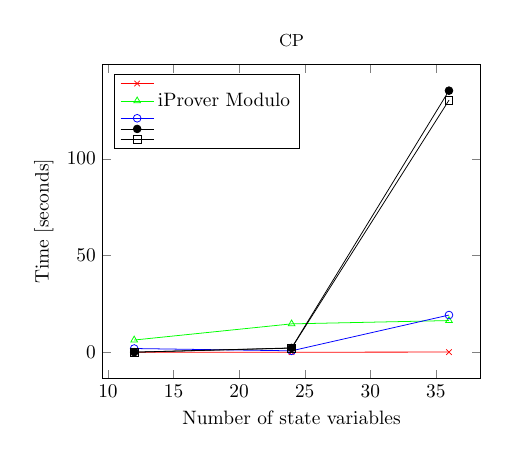
\begin{tikzpicture}[scale=0.7]
		\begin{axis}[title={\small{CP}},legend pos=north west, 
		% small,
		xlabel = {\normalsize Number of state variables},
		ylabel = {\normalsize Time [seconds]}
		]
		\addplot [color=red, mark=x] coordinates
		{
			(12,0.011)
			(24,0.010)
			(36,0.057)     
		};
		\addplot [color=green, mark=triangle] coordinates
		{
			(12,6.293)
			(24,14.648)
			(36,16.351)
		};
		\addplot [color=blue, mark=o] coordinates
		{
			(12,1.904)
			(24,0.714)
			(36,19.200)
		};
		\addplot [color=black,mark=*] coordinates
		{
			(12,0.014)
			(24,2.202)
			(36,135.202)
		};
		\addplot [color=black,mark=square] coordinates
		{
			(12,0.018)
			(24,2.100)
			(36,130.268)
		};
		{\legend{\sctl{},\tool{iProver Modulo}, \verds{}, \nusmv{}, \nuxmv{}}}
		\end{axis}
		\end{tikzpicture}
		
	\end{tabular}
	%		\end{subfigure}
	%		\begin{subfigure}
	%			\centering
	\begin{tabular}{c}
		\scriptsize
		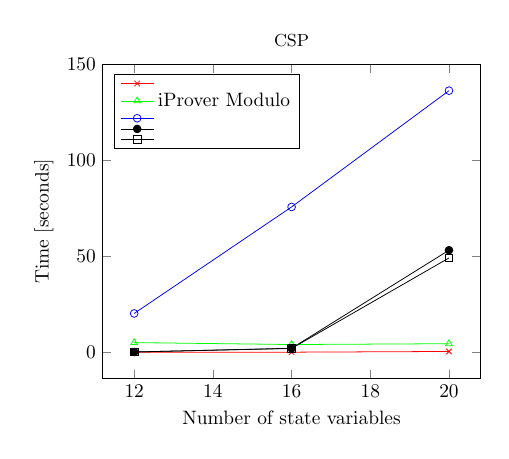
\begin{tikzpicture}[scale=0.7]
		\begin{axis}[title={\small{CSP}},legend pos=north west, 
		%small,
		xlabel = {\normalsize Number of state variables},
		ylabel = {\normalsize Time [seconds]}
		]
		\addplot [color=red, mark=x] coordinates
		{
			(12,0.006)
			(16,0.007)
			(20,0.374)      
		};
		\addplot [color=green, mark=triangle] coordinates
		{
			(12,4.995)
			(16,3.997)
			(20,4.424)
		};
		\addplot [color=blue, mark=o] coordinates
		{
			(12,20.203)
			(16,75.741)
			(20,136.387)
		};
		\addplot [color=black,mark=*] coordinates
		{
			(12,0.105)
			(16,2.036)
			(20,53.195)
		};
		\addplot [color=black,mark=square] coordinates
		{
			(12,0.107)
			(16,1.957)
			(20,49.144)
		};
		{\legend{\sctl{},\tool{iProver Modulo}, \verds{}, \nusmv{}, \nuxmv{}}}
		\end{axis}
		\end{tikzpicture}
	\end{tabular}
	%		\end{subfigure}
	
	\caption{在测试集一上各个工具的平均占用时间}
	\label{fig:average_time}
\end{figure}

\begin{figure}[h!]\centering
	%	\begin{subfigure}\centering
	\begin{tabular}{c}
		\scriptsize
		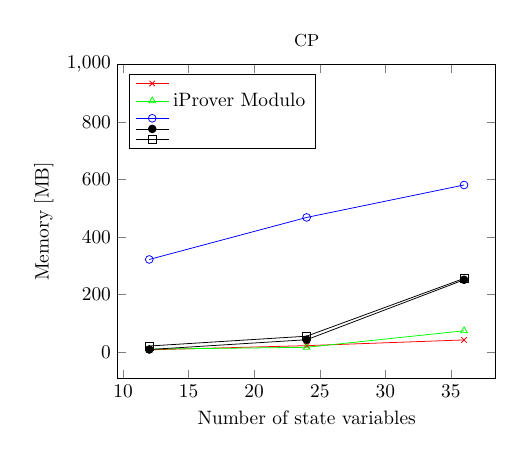
\begin{tikzpicture}[scale=0.7]
		\begin{axis}[title={\small{CP}},legend pos=north west, 
		%small, 
		ymax=1000,
		xlabel = {\normalsize Number of state variables},
		ylabel = {\normalsize Memory [MB]}
		]
		\addplot [color=red, mark=x] coordinates
		{
			(12,7.845)
			(24,22.328)
			(36,42.184)     
		};
		\addplot [color=green, mark=triangle] coordinates
		{
			(12,10.111)
			(24,16.547)
			(36,73.946)
		};
		\addplot [color=blue, mark=o] coordinates
		{
			(12,322.020)
			(24,468.169)
			(36,581.011)
		};
		\addplot [color=black,mark=*] coordinates
		{
			(12,8.818)
			(24,42.924)
			(36,251.364)
		};
		\addplot [color=black,mark=square] coordinates
		{
			(12,21.013)
			(24,55.179)
			(36,256.058)
		};
		\legend{\sctl{},\tool{iProver Modulo}, \verds{}, \nusmv{}, \nuxmv{}}
		\end{axis}
		\end{tikzpicture}
		
	\end{tabular}
	%	\end{subfigure}
	%	\begin{subfigure}
	%		\centering
	\begin{tabular}{c}
		\scriptsize
		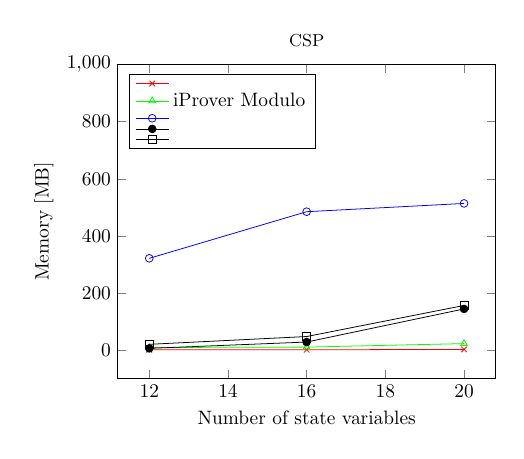
\begin{tikzpicture}[scale=0.7]
		\begin{axis}[title={\small{CSP}},legend pos=north west, 
		%small, 
		ymax=1000,
		xlabel = {\normalsize Number of state variables},
		ylabel = {\normalsize Memory [MB]}
		]
		\addplot [color=red, mark=x] coordinates
		{
			(12,1.984)
			(16,2.039)
			(20,3.383)      
		};
		\addplot [color=green, mark=triangle] coordinates
		{
			(12,10.070)
			(16,11.449)
			(20,23.660)
		};
		\addplot [color=blue, mark=o] coordinates
		{
			(12,322.023)
			(16,485.081)
			(20,514.027)
		};
		\addplot [color=black,mark=*] coordinates
		{
			(12,7.051)
			(16,29.151)
			(20,144.974)
		};
		\addplot [color=black,mark=square] coordinates
		{
			(12,21.168)
			(16,48.423)
			(20,157.113)
		};
		{\legend{\sctl{},\tool{iProver Modulo}, \verds{}, \nusmv{}, \nuxmv{}}}
		\end{axis}
		\end{tikzpicture}
	\end{tabular}
	%	\end{subfigure}
	
	\caption{在测试集一上各个工具的平均占用内存}
	\label{fig:average_memory}
\end{figure}
}

\paragraph{测试集二的实验结果}
由表\ref{tabl:solvable:extended}与表\ref{tabl:compare:extended}可知:在测试集二的5760个测试用例中,\tool{iProver Modulo}、\verds{}、\nusmv{}、\nuxmv{}、\sctlprov{}分别能验证2748(44.7\%)、2226(38.6\%)、728(12.6\%)、736(12.8\%)、4441(77.1\%)个测试用例;同时\sctlprov{}分别在4441(77.1\%)、4438(77.0\%)、4432(76.9\%)、4432(76.9\%)个测试用例上占用时间和空间少于\tool{iProver Modulo}、\verds{}、\nusmv{}、\nuxmv{}。各个工具的时间占用随着状态变量的个数的变化趋势如图\ref{fig:average_time:extended}所示;各个工具占用空间随着状态变量的个数的变化趋势如图\ref{fig:average_memory:extended}所示。

\begin{table}[!h]\small
	%	\begin{tabular}{c c}
	%\renewcommand{\arraystretch}{1.0}
	%		\begin{minipage}[b]{0.55\linewidth}
	\centering
	\setlength{\tabcolsep}{3pt}
	\begin{tabular}{| l | r | r | r | r | r |}
		\hline
		\textbf{程序类型} & \tool{iProver Modulo} & \verds{} & \nuxmv{} & \nuxmv{} & \sctl{} \\
		\hline
		\code{CP ($b = 48$)} & 375(78.1\%) & 400(83.3\%) & 171(35.6\%) & 176(36.7\%) & 446(92.9\%)  \\
		\hline
		\code{CP ($b = 60$)} & 360(75.0\%) & 403(84.0\%) & 22(4.6\%) & 23(4.8\%) & 440(91.7\%)  \\
		\hline
		\code{CP ($b = 72$)} & 347(72.3\%) & 383(79.8\%) &  0 & 0 & 437(91.0\%)  \\
		\hline
		\code{CP ($b=252$)} & 299(62.3\%) & 216(45.0\%) & 0 & 0 & 371(77.3\%) \\
		\hline
		\code{CP ($b=504$)} & 292(60.8\%) & 0 & 0 & 0 & 335(69.8\%)\\
		\hline
		\code{CP ($b=1008$)} & 271(56.5\%) & 0 & 0 & 0 & 278(57.9\%)\\
		
		\hline
		\code{CSP ($b=24$)} & 190(39.6\%) & 235(49.0\%) &  421(87.7\%) & 423(88.1\%) & 430(89.6\%) \\
		\hline
		\code{CSP ($b=28$)} & 172(35.8\%) & 229(47.7\%) & 106(22.1\%) & 108(22.5\%) & 426(88.8\%) \\
		\hline
		\code{CSP ($b=32$)} & 158(32.9\%) & 224(46.7\%) & 8(1.7\%) & 6(1.3\%) & 418(87.1\%) \\
		
		\hline
		\code{CSP ($b=252$)} & 114(23.6\%) & 136(28.3\%) & 0 & 0 & 312(65.0\%) \\
		\hline
		\code{CSP ($b=504$)} & 108(22.5\%) & 0 & 0 & 0 & 295(61.5\%) \\
		\hline
		\code{CSP ($b=1008$)} & 62(12.9\%) & 0 & 0 & 0 & 253(52.7\%)\\
		\hline
		Sum & 2748(47.7\%) & 2226(38.6\%) & 728(12.6\%) & 736(12.8\%) & 4441(77.1\%)\\
		\hline
	\end{tabular}
	\tabcaption{测试集二中5个工具能成功验证的测试用例个数}
	\label{tabl:solvable:extended}
	\vspace{0.5cm}
	%		\end{minipage}
	%		&
\end{table}

\begin{table}[h!]\small
	%\setlength{\tabcolsep}{3pt}
	%\renewcommand{\arraystretch}{1.0}
	%		\begin{minipage}[b]{0.45\linewidth}
	%			\centering
	%			\setlength{\tabcolsep}{3pt}
	\centering
	\setlength{\tabcolsep}{3pt}
	\begin{tabular}{| l | r | r | r | r |}
		\hline
		\textbf{程序类型} & \tool{iProver Modulo} & \verds{} & \nusmv{} & \nuxmv{}\\
		\hline
		\code{CP ($b=48$)} & 446(92.9\%) & 444(92.5\%) & 442(92.1\%) & 442(92.1\%) \\
		\hline
		\code{CP ($b=60$)} & 440(91.7\%) & 440(91.7\%) & 440(91.7\%) & 440(91.7\%) \\
		\hline
		\code{CP ($b=72$)} & 437(91.0\%) & 437(91.0\%) & 437(91.0\%) & 437(91.0\%) \\
		\hline
		\code{CP ($b=252$)} & 371(77.3\%) & 371(77.3\%) & 371(77.3\%) & 371(77.3\%)\\
		\hline
		\code{CP ($b=504$)} & 335(69.8\%) & 335(69.8\%) & 335(69.8\%) & 335(69.8\%)\\
		\hline
		\code{CP ($b=1008$)} & 278(57.9\%) & 278(57.9\%) & 278(57.9\%) & 278(57.9\%)\\
		\hline
		\code{CSP ($b=24$)} & 430(89.6\%) & 429(89.4\%) & 426(88.8\%) & 426(88.8\%) \\
		\hline
		\code{CSP ($b=28$)} & 426(88.8\%) & 426(88.8\%) & 425(88.5\%) & 425(88.5\%) \\
		\hline
		\code{CSP ($b=32$)} & 418(87.1\%) & 418(87.1\%) & 418(87.1\%) & 418(87.1\%) \\
		\hline
		\code{CSP ($b=252$)} & 312(65.0\%) & 312(65.0\%) & 312(65.0\%) & 312(65.0\%)\\
		\hline
		\code{CSP ($b=504$)} & 295(61.5\%) & 295(61.5\%) & 295(61.5\%) & 295(61.5\%)\\
		\hline
		\code{CSP ($b=1008$)} & 253(52.7\%) & 253(52.7\%) & 253(52.7\%) & 253(52.7\%)\\
		\hline
		Sum & 4441(77.1\%) & 4438(77.0\%) & 4432(76.9\%) & 4432(76.9\%)\\
		\hline
	\end{tabular}	
	\tabcaption{测试集二中\sctl{}相比其他工具占用资源(时间和空间)少的测试用例个数}
	\label{tabl:compare:extended}
	%		\end{minipage}
	%	\end{tabular}
\end{table}


\begin{figure}[h!]\centering
	%	\begin{subfigure}\centering
	\begin{tabular}{c}			
		\scriptsize
		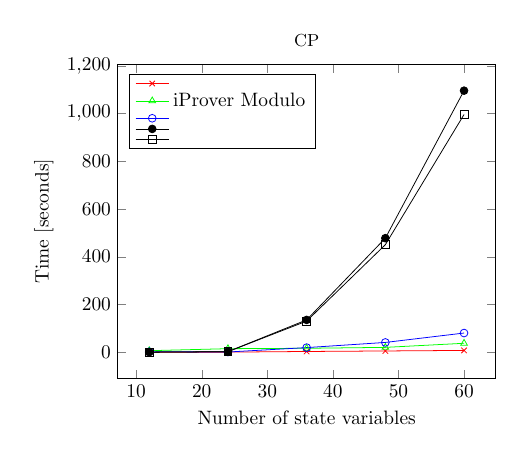
\begin{tikzpicture}[scale=0.7]
		\begin{axis}[title={\small{CP}},legend pos=north west, 
		%small,
		xlabel = {\normalsize Number of state variables},
		ylabel = {\normalsize Time [seconds]}
		]
		\addplot [color=red, mark=x] coordinates
		{
			(12,0.011)
			(24,0.280)
			(36,2.929)  
			(48,5.100)
			(60,7.357)   
		};
		\addplot [color=green, mark=triangle] coordinates
		{
			(12,6.293)
			(24,14.648)
			(36,16.351)
			(48,20.130)
			(60,37.303) 
		};
		\addplot [color=blue, mark=o] coordinates
		{
			(12,1.904)
			(24,0.714)
			(36,19.200)
			(48,40.825)
			(60,80.201)
		};
		\addplot [color=black,mark=*] coordinates
		{
			(12,0.014)
			(24,2.202)
			(36,135.202)
			(48,477.578)
			(60,1095.582)
		};
		\addplot [color=black,mark=square] coordinates
		{
			(12,0.018)
			(24,2.100)
			(36,130.268)
			(48,450.324)
			(60,995.689)
		};
		\legend{\sctl{}, \tool{iProver Modulo}, \verds{}, \nusmv{}, \nuxmv{}}
		\end{axis}
		\end{tikzpicture}
		
	\end{tabular}
	%	\end{subfigure}
	%	\begin{subfigure}
	%		\centering
	\begin{tabular}{c}
		\scriptsize
		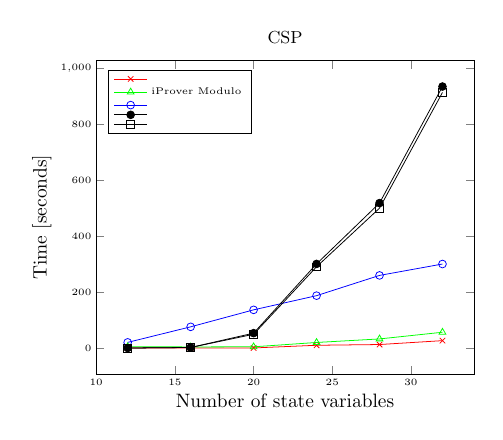
\begin{tikzpicture}[scale=0.7]
		\begin{axis}[title={\small{CSP}},legend pos=north west, 
		%small,
		xlabel = {\normalsize Number of state variables},
		ylabel = {\normalsize Time [seconds]}
		]
		\addplot [color=red, mark=x] coordinates
		{
			(12,0.006)
			(16,0.007)
			(20,0.374) 
			(24,9.903)
			(28,12.548)
			(32,26.417)     
		};
		\addplot [color=green, mark=triangle] coordinates
		{
			(12,4.995)
			(16,3.997)
			(20,4.424)
			(24,19.903)
			(28,32.548)
			(32,56.417)   
		};
		\addplot [color=blue, mark=o] coordinates
		{
			(12,20.203)
			(16,75.741)
			(20,136.387)
			(24,187.043)
			(28,259.342)
			(32,300.031)
		};
		\addplot [color=black,mark=*] coordinates
		{
			(12,0.105)
			(16,2.036)
			(20,53.195)
			(24,300.406)
			(28,517.544)
			(32,933.722)
			
		};
		\addplot [color=black,mark=square] coordinates
		{
			(12,0.107)
			(16,1.957)
			(20,49.144)
			(24,290.205)
			(28,499.454)
			(32,912.527)
		};
		\tiny{\legend{\sctl{}, \tool{iProver Modulo}, \verds{}, \nusmv{}, \nuxmv{}}}
		\end{axis}
		\end{tikzpicture}
	\end{tabular}
	%	\end{subfigure}
	
	\caption{在测试集一、二上各个工具的平均占用时间}
	\label{fig:average_time:extended}
\end{figure}

\begin{figure}[h!]\centering
	\scriptsize
	%	\begin{subfigure}\centering
	\begin{tabular}{c}
		
		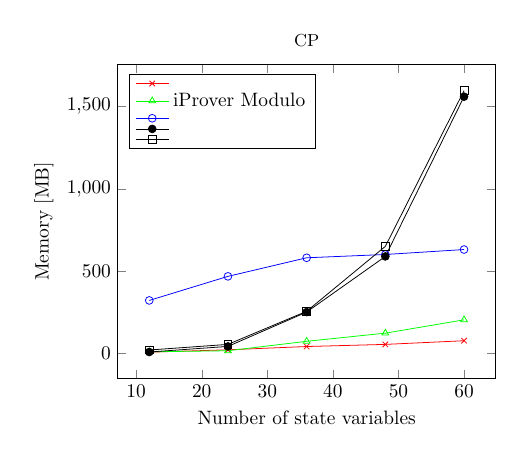
\begin{tikzpicture}[scale=0.7]
		\begin{axis}[title={\small{CP}},legend pos=north west, 
		%small,
		xlabel = {\normalsize Number of state variables},
		ylabel = {\normalsize Memory [MB]}
		]
		\addplot [color=red, mark=x] coordinates
		{
			(12,7.845)
			(24,22.328)
			(36,42.184)  
			(48,55.100)
			(60,77.357)   
		};
		\addplot [color=green, mark=triangle] coordinates
		{
			(12,10.111)
			(24,16.547)
			(36,73.946)
			(48,123.342)
			(60,204.298)
		};
		\addplot [color=blue, mark=o] coordinates
		{
			(12,322.020)
			(24,468.169)
			(36,581.011)
			(48,601.023)
			(60,631.034)
		};
		\addplot [color=black,mark=*] coordinates
		{
			(12,8.818)
			(24,42.924)
			(36,251.364)
			(48,589.205)
			(60,1559.283)
		};
		\addplot [color=black,mark=square] coordinates
		{
			(12,21.013)
			(24,55.179)
			(36,256.058)
			(48,650.324)
			(60,1595.689)
		};
		\legend{\sctl{}, \tool{iProver Modulo}, \verds{}, \nusmv{}, \nuxmv{}}
		\end{axis}
		\end{tikzpicture}
		
	\end{tabular}
	%	\end{subfigure}
	%	\begin{subfigure}
	%		\centering
	\begin{tabular}{c}
		\scriptsize
		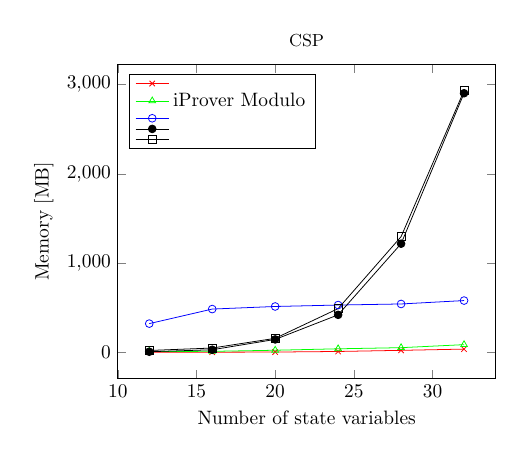
\begin{tikzpicture}[scale=0.7]
		\begin{axis}[title={\small{CSP}},legend pos=north west, 
		%small,
		xlabel = {\normalsize Number of state variables},
		ylabel = {\normalsize Memory [MB]}
		]
		\addplot [color=red, mark=x] coordinates
		{
			(12,1.984)
			(16,2.039)
			(20,3.383) 
			(24,9.903)
			(28,22.548)
			(32,36.417)     
		};
		\addplot [color=green, mark=triangle] coordinates
		{
			(12,10.070)
			(16,11.449)
			(20,23.660)
			(24,39.903)
			(28,52.548)
			(32,86.417)
		};
		\addplot [color=blue, mark=o] coordinates
		{
			(12,322.023)
			(16,485.081)
			(20,514.027)
			(24,530.238)
			(28,542.231)
			(32,580.357)
		};
		\addplot [color=black,mark=*] coordinates
		{
			(12,7.051)
			(16,29.151)
			(20,144.974)
			(24,420.406)
			(28,1217.544)
			(32,2903.722)
			
		};
		\addplot [color=black,mark=square] coordinates
		{
			(12,21.168)
			(16,48.423)
			(20,157.113)
			(24,490.205)
			(28,1296.454)
			(32,2932.527)
		};
		{\legend{\sctl{}, \tool{iProver Modulo}, \verds{}, \nusmv{}, \nuxmv{}}}
		\end{axis}
		\end{tikzpicture}
	\end{tabular}
	%	\end{subfigure}
	
	\caption{在测试集一、二上各个工具的平均占用内存}
	\label{fig:average_memory:extended}
\end{figure}

\couic{
	\paragraph{测试集三的实验结果}
	由表\ref{tabl:solvable:larger}可知:在测试集三的2880个测试用例中,\tool{iProver Modulo}、\verds{}、\sctlprov{}分别能验证1146(39.8\%)、352(12.2\%)、1844(64.0\%)个测试用例,然而\nusmv{}与\nuxmv{}无法验证本测试集中的测试用例。
	\couic{For 2880 test cases in this benchmark, \tool{iProver Modulo} can solve 1146 (39.8\%) cases, \verds{} can solve 352 (12.2\%) cases, \sctl{} can solve 1844 (64.0\%) cases, while neither \nusmv{} nor \nuxmv{} can solve any case.}
	
	
	\begin{table}[h]\small
		\setlength{\tabcolsep}{3pt}
		%\renewcommand{\arraystretch}{1.0}
		\begin{center}
			\begin{tabular}{| l | r | r | r | r | r |}
				\hline
				\textbf{Programs} & \tool{iProver Modulo} & \verds{} &
				\nusmv{} & \nuxmv{} & \sctl{} \\
				\hline
				\code{CP ($b=252$)} & 299(62.3\%) & 216(45.0\%) & 0 & 0 & 371(77.3\%) \\
				\hline
				\code{CP ($b=504$)} & 292(60.8\%) & 0 & 0 & 0 & 335(69.8\%)\\
				\hline
				\code{CP ($b=1008$)} & 271(56.5\%) & 0 & 0 & 0 & 278(57.9\%)\\
				
				\hline
				\code{CSP ($b=252$)} & 114(23.6\%) & 136(28.3\%) & 0 & 0 & 312(65.0\%) \\
				\hline
				\code{CSP ($b=504$)} & 108(22.5\%) & 0 & 0 & 0 & 295(61.5\%) \\
				\hline
				\code{CSP ($b=1008$)} & 62(12.9\%) & 0 & 0 & 0 & 253(52.7\%)\\
				\hline
				Sum & 1146(39.8\%) & 352(12.2\%) & 0 & 0 & 1844(64.0\%)\\ \hline
			\end{tabular}
		\end{center}
		\tabcaption{测试集三中5个工具能成功验证的测试用例个数}
		\label{tabl:solvable:larger}
	\end{table}
}

\subsubsection{连续 vs. 递归}
传统的即时模型检测工具通常使用递归算法来进行公式的证明和状态空间的搜索。不同于递归算法,\sctlprov{}的验证算法是连续传递风格(Continuation-Passing Style,简称CPS),CPS的应用可以大大减少栈的操作,从而节省验证所需的时间。为了对比使用连续传递风格的算法和递归算法的效率,我们对比了\sctlprov{}和\sctlprovr{}分别在测试集一、二上的实验数据。其中\sctlprovr{}与\sctlprov{}的唯一不同是使用递归算法来证明公式和搜索状态空间。如表\ref{tabl:cont_vs_rec}所示,\sctlprov{}能成功验证的测试用例个数比\sctlprovr{}多10\%,而且\sctlprov{}在绝大多数能成功运行的测试用例中比\sctlprovr{}所用时间短。如图\ref{fig:average_time:recursive:vs:continuation}所示,随着状态变量数的增加,\sctlprovr{}的平均运行时间多于\sctlprov{},而且时间的变化幅度更大。


{
	\begin{figure}[h!]\small
		\setlength{\tabcolsep}{1pt}
		\begin{center}
			\begin{tabular}{| l | r | r | r |}
				
				\hline
				%				\textbf{Bench} & \sctl{} solvable & \sctlprovr{} solvable & t(\sctlprov) $<$ t(\sctlprovr{})  \\
				\multirow{2}{*}{\textbf{测试集}} & \multicolumn{2}{c|}{Solvable} &\multirow{2}{*}{ t(\sctlprov) $<$ t(\sctlprovr{})}\\
				\cline{2-3}
				{}&\sctl{}&\sctlprovr{}&{}\\
				\hline
				%\code{CP} & 1430(99.3\%) & 1354(94.0\%) \\
				%\hline
				%\code{CSP} & 1432(99.4\%) & 1328(92.2\%) \\
				%\hline
				\textbf{一} & 2862(99.4\%) & 2682(93.1\%) & 2598(90.2\%)\\
				\hline
				\textbf{二} & 4446(77.2\%) & 3826(66.4\%) & 3841(71.9\%)\\
				%				\textbf{\#2} & 2597(90.2\%) & 2306(80.1\%) & 2406(83.5\%)\\
				%				\hline
				%				\textbf{\#3} & 1849(64.2\%) & 1520(52.8\%) & 1735(60.2\%)\\
				\hline
			\end{tabular}
		\end{center}
		\tabcaption{在测试集一、二上\sctl{}和\sctlprovr{}的实验数据对比}
		\label{tabl:cont_vs_rec}
	\end{figure}
}


\begin{figure}[h!]\centering
	%	\begin{subfigure}\centering
	\begin{tabular}{c}
		\scriptsize
		\begin{tikzpicture}[scale=0.7]
		\begin{axis}[title={\small{CP}},legend pos=north west, 
		%small,
		xlabel = {\normalsize Number of state variables},
		ylabel = {\normalsize Time [seconds]}
		]
		\addplot [color=red, mark=x] coordinates
		{
			(12,0.011)
			(24,0.280)
			(36,2.929)  
			(48,5.100)
			(60,7.357)
			(72,19.566)   
		};
		\addplot [color=black,mark=*] coordinates
		{
			(12,0.032)
			(24,2.238)
			(36,6.717)
			(48,17.578)
			(60,55.582)
			(72,101.265)
		};
		\legend{\sctlprov, \sctlprovr{}}
		\end{axis}
		\end{tikzpicture}
		
	\end{tabular}
	%	\end{subfigure}
	%	\begin{subfigure}
	\centering
	\begin{tabular}{c}
		\scriptsize
		\begin{tikzpicture}[scale=0.7]
		\begin{axis}[title={\small{CSP}},legend pos=north west, 
		%small,
		xlabel = {\normalsize Number of state variables},
		ylabel = {\normalsize Time [seconds]}
		]
		\addplot [color=red, mark=x] coordinates
		{
			(12,0.006)
			(16,0.007)
			(20,0.374) 
			(24,9.903)
			(28,12.548)
			(32,26.417)
			(52,91.134)
			(72,180.098)     
		};
		
		\addplot [color=black,mark=*] coordinates
		{
			(12,0.035)
			(16,1.238)
			(20,10.717)
			(24,30.406)
			(28,57.544)
			(32,83.722)
			(52,234.546)
			(72,504.256) 
			
		};
		{\legend{\sctlprov,\sctlprovr{}}}
		\end{axis}
		\end{tikzpicture}
	\end{tabular}
	%	\end{subfigure}
	
	\caption{\sctl{}和\sctlprovr{}平均运行时间}
	\label{fig:average_time:recursive:vs:continuation}
\end{figure}


\subsection{公平性性质的验证}\label{subsec:fair}
在本小节,我们来对比\sctlprov{}和\verds{}、\nusmv{}、\nuxmv{}在验证公平性性质时的效率。此次对比没有考虑\tool{iProver Modulo},这是因为\tool{iProver Modulo}无法验证公平性性质。此次对比所用的所有测试用例(测试集四)同样分为两种:互斥算法和环算法\footnote{\url{http://lcs.ios.ac.cn/~zwh/verds/verds_code/bp12.rar}}。下面我们介绍这两种测试用例。


\couic{In this part, we evaluate benchmark \#4, which models mutual exclusion
	algorithms and ring
	algorithms\footnote{\url{http://lcs.ios.ac.cn/~zwh/verds/verds_code/bp12.rar}}.
	Then, we compare the evaluation results of \sctl{}, \verds{},
	\nusmv{}, and \nuxmv{}, and we do not consider \tool{iProver Modulo}
	because \tool{iProver Modulo} cannot handle \CTL{} properties with
	fairness constraints \cite{Ji15}.}


\subsubsection{测试集三}
测试集三种包含两类测试用例:互斥算法和环算法。

每个互斥算法包含$n$个进程,$n$个进程的调度方式如下:对于$0\le i\le n-2$,进程$i+1$的迁移在进程$i$之后,进程$0$的迁移在进程$n-1$之后。
互斥算法中$n$的取值范围为$\{6,...,51\}$。
要验证的性质如表\ref{tabl:mutual:properties}所示,其中$non_i$,$try_i$以及$cri_i$分别表示进程$i$的内部状态为\textsf{noncritical},\textsf{trying}以及\textsf{critical}。
所有的性质必须在公平性的前提下进行验证,即在互斥算法的执行过程中没有进程饿死(永远处在等待状态)。

\begin{table}[h!]
	\small
	%\setlength{\tabcolsep}{3pt}
	%\renewcommand{\arraystretch}{1.0}
	\begin{center}
		\begin{tabular}{| l | l |}
			\hline
			\textbf{性质} & \textbf{互斥算法公式}\\
			\hline
			{$P_1$} & $EF (cri_0 \wedge cri_1)$  \\
			\hline
			{$P_2$} &  $AG (try_0 \Rightarrow AF (cri_0))$\\
			\hline
			{$P_3$} &  $AG (try_1 \Rightarrow AF (cri_1))$\\
			
			\hline
			{$P_4$} &  $AG (cri_0 \Rightarrow A cri_0 U (\neg cri_0 \wedge A \neg cri_0 U cri_1))$  \\
			\hline
			{$P_5$} &  $AG (cri_1 \Rightarrow A cri_1 U (\neg cri_1 \wedge A \neg cri_1 U cri_0))$\\
			\hline
		\end{tabular}
	\end{center}
	\figcaption{互斥算法的性质}
	\label{tabl:mutual:properties}
\end{table}

每个环算法包含$n$个进程,$n$个进程的调度方式如下:对于$1\le i\le n-1$,进程$i$的内部状态由进程$i-1$的输出决定,进程$0$的内部状态由进程$n-1$的输出决定;每个进程的输出取决于它的内部状态;每个进程的内部状态由5个布尔变量的值表示;每个进程的输出由1个布尔变量表示。
环算法中$n$的取值范围为$\{3,...,10\}$。
要验证的性质如表\ref{tabl:ring:properties}所示,其中$out_i$表示进程$i$的输出为布尔值\textsf{true}。
所有的性质必须在公平性的前提下进行验证,即在环算法的执行过程中没有进程饿死(永远处在等待状态)。

\begin{table}[h!]
	\small
	%\setlength{\tabcolsep}{3pt}
	%\renewcommand{\arraystretch}{1.0}
	\begin{center}
		\begin{tabular}{| l | l |}
			\hline
			\textbf{性质} & \textbf{环算法公式}\\
			\hline
			{$P_1$} & $AGAF out_0 \wedge AGAF \neg out_0$ \\
			\hline
			{$P_2$} &  $AGEF out_0 \wedge AGEF \neg out_0$ \\
			\hline
			{$P_3$} &  $EGAF out_0 \wedge EGAF \neg out_0$\\
			
			\hline
			{$P_4$} &  $EGEF out_0 \wedge EGEF \neg out_0$ \\
			\hline
		\end{tabular}
	\end{center}
	\figcaption{环算法的性质}
	\label{tabl:ring:properties}
\end{table}

%	The experimental results are shown in Table~\ref{tabl:solvable:mutual:ring}, \ref{tabl:compare:mutual:ring}, and \ref{tabl:data:mutual:ring}. 
\couic{
	如表\ref{tabl:solvable:mutual:ring}、表\ref{tabl:compare:mutual:ring}、表\ref{tabl:data:mutual}、表\ref{tabl:data:ring}所示:\sctl{}成功验证的测试用例个数多于\verds, \nusmv{}以及\nuxmv{};同时在超过75\%的测试用例中,\sctl{}占用资源(时间和空间)相比另外三个工具更少。
	
	\paragraph{Experimental data for benchmark \#3.}
	For 262 test cases in this benchmark, \verds{} can solve 152 (58.0\%) cases, both \nusmv{} and \nuxmv{} can solve 71 (27.1\%) cases, and \sctlprov{} can solve 211 (80.2\%) cases (Table \ref{tabl:solvable:mutual:ring}). The number of test cases where \sctlprov{} runs faster and used less memory are 200 (76.3\%) comparing with \verds{}, and 211 (80.2\%) comparing both with \nusmv{} and with \nuxmv{} (Table \ref{tabl:solvable:mutual:ring}).
}

\paragraph{测试集三的实验结果} 
如表\ref{tabl:solvable:mutual:ring}所示,在本测试集的262个测试用例中,\verds{}、\nusmv{}、\nuxmv{}、\sctlprov{}分别能解决152 (58.0\%)、71 (27.1\%)、71 (27.1\%)、211 (80.2\%)个测试用例。如表\ref{tabl:compare:mutual:ring}所示,\sctlprov{}分别在200 (76.3\%)、211 (80.2\%)、211 (80.2\%)个测试用例上占用的时间和空间少于\verds{}、\nusmv{}、\nuxmv{}。测试集三上各个工具的详细实验数据如附录\ref{appendix:detail:data}中表\ref{tabl:data:mutual}和表\ref{tabl:data:ring}所示。

\begin{figure}[h!]
	\small
	%\setlength{\tabcolsep}{3pt}
	%\renewcommand{\arraystretch}{1.0}
	%	\begin{tabular}{c c}
	%		\begin{minipage}[b]{0.45\linewidth}
	\centering
	\setlength{\tabcolsep}{3pt}
	\begin{tabular}{| l | r | r | r | r |}
		\hline
		\textbf{程序类型} & \verds{} & \nusmv{} & \nuxmv{} &  \sctl{} \\
		\hline
		{互斥算法} & 136 (59.1\%) & 50 (21.7\%) & 50 (21.7\%) & 191 (83.0\%)  \\
		\hline
		{环算法} & 16 (50.0\%) & 21 (65.6\%) & 21 (65.6\%) & 20 (62.5\%) \\
		\hline
		总和 & 152(58.0\%) & 71(27.1\%) & 71(27.1\%) & 211 (80.5\%)\\
		\hline
	\end{tabular}	
	\tabcaption{测试集三中各个工具能成功验证的测试用例的个数}
	\label{tabl:solvable:mutual:ring}
	\vspace{0.5cm}
\end{figure}
\begin{figure}[h!]
	\small
	%\scriptsize
	%			\centering
	%			\setlength{\tabcolsep}{3pt}
	\centering
	\setlength{\tabcolsep}{3pt}
	\begin{tabular}{| l | r | r | r |}
		\hline
		\textbf{程序类型} & \verds{} & \nusmv{} & \nuxmv{}  \\
		\hline
		{互斥算法} & 187 (81.3\%) & 191 (83.0\%) & 191 (83.0\%)   \\
		\hline
		{环算法} & 13 (40.6\%) & 20 (62.5\%) & 20 (62.5\%)  \\
		\hline
		总和 & 200(76.3\%) & 211(80.5\%) & 211(80.5\%) \\
		\hline
	\end{tabular}
	\tabcaption{测试集三中\sctl{}占用资源更少的的测试用例的个数}
	\label{tabl:compare:mutual:ring}
	%		\end{minipage}
	%	\end{tabular}
\end{figure}

\subsection{工业级测试用例的验证}	\label{subsc:vlts}
在本小节中,我们在工业级测试用例上(测试集四)对比\sctl{}与其他工具的效率。不同于测试集一、二、三,本次对比所用的测试用例均为符号迁移系统(Labeled Transition System,简称\textsf{LTS}),而且所有的\textsf{LTS}均以\textsf{BCG}(Binary-Coded Graph)格式表示,其中\textsf{BCG}格式可以用来表示较大的状态空间。测试集四是形式化验证工具包\CADP{}\cite{GaravelLMS13}的一部分,也被称作\textsf{VLTS}(Very Large Transition Systems)测试集。
不同于本文中其他的形式化验证工具,\CADP{}是专门验证基于动作的形式化系统的工具,比如符号迁移系统、马尔可夫链等。
测试集四中的例子均由对不同的传输协议以及并发系统的建模而得到的,其中许多例子是对工业级系统的建模\footnote{\url{http://cadp.inria.fr/resources/vlts/}}。

测试集四中共有40个测试用例,针对每个测试用例我们分别验证有无死锁与活锁。由于\sctlprov{}是基于Kripke模型的验证工具,因此在验证之前,我们需将每个\textsf{LTS}转换到相应的Kripke模型,然后在转换后的Kripke模型中进行验证。


给定一个\textsf{LTS} $\mathcal{L} = \langle s_0, S, Act, \rightarrow \rangle$,其中$s_0$是初始状态;$s$是一个有穷的状态集合;$Act$是一个有穷的动作集合;$\rightarrow \subseteq S\times Act\times S$是迁移规则。那么$\mathcal{L}$到相应的Kripke模型$\mathcal{M} = \langle s_0', S', \lra, {\mathcal P} \rangle$的转换过程如下:

\begin{itemize}
	\item 令$s_0'$为$(s_0, \cdot)$,其中$\cdot\notin Act$是一个特殊的动作符号。
	\item 分别将$(s_d,\cdot)$与$S'$与$(s_d,\cdot)\lra (s_d,\cdot)$添加到$S'$与$\lra$中,其中$(s_d,\cdot)$区分于$S'$中的所有其他状态。
	\item 重复以下步骤直到没有更多的状态和迁移被添加到$\mathcal{M}$中:
	\begin{itemize}
		\item 如果$\cal L$中存在一个迁移$s_1\stackrel{a}\rightarrow s_2$,那么对于所有的$(s_1, b)\in S'$,将$(s_1, b)\lra (s_2, a)$添加到$\cal M$的迁移关系$\lra$中,其中$a, b\in Act\cup\{\cdot\}$;同时将$(s_2, a)$添加到$\cal M$的状态集合$S'$中;
		\item 对于$S'$中的状态$(s,a)$,如果$s$在$\cal L$中没有后继,那么将$(s,a)\lra (s_d,\cdot)$添加到$\cal M$的迁移关系$\lra$。
	\end{itemize}
	\item 最后,令$P=\{(s_d,\cdot)\}$而且$Q = \{(s,a)\mid s\in S\wedge a=\tau\}$。
\end{itemize}
经过从\textsf{LTS}到Kripke模型的转换之后,我们就可以在\sctlprov{}中验证死锁与活锁的存在了。

\paragraph{死锁}
在\textsf{LTS}中,死锁状态指的是没有后继的状态。当验证一个\textsf{LTS} $\cal L$中是否存在可达的死锁状态时,我们首先将$\cal L$经过以上的转换方法转换到一个Kripke模型$\cal M$。经过观察得知,$\cal L$中存在一个可达的死锁状态当且仅当$\cal M$中状态$(s_d,\cdot)$时可达的。

然后,我们可以通过证明如下的公式来验证$\cal M$中$(s_d,\cdot)$是否可达:
$$EF_x(P(x))((s_0,\cdot))$$ 

这个公式是可证的当且仅当$\cal M$中存在一条形式为$(s_0,\cdot)\lra^*(s,a)\lra (s_d,\cdot)$的路径,其中$a$是一个动作符号,而且$s$在$\mathcal{L}$中没有后继。
因此,这个公式可以被用来验证$\cal L$中有没有可达的死锁状态。 

\paragraph{活锁}
在\textsf{LTS}中,活锁指的是所有动作均为$\tau$的无穷的环状路径。在\textsf{LTS}中检测活锁相比检测死锁更复杂,原因是当观察一个迁移的时候,状态和动作都要考察到。
与在检测死锁的方法一样,当验证一个\textsf{LTS} $\cal L$中是否存在可达的活锁时,我们首先将$\cal L$经过以上的转换方法转换到一个Kripke模型$\cal M$。通过以下分析可知,
$\cal L$中存在一个可达的活锁当且仅当$\cal M$中存在一个环状路径,而且该路径上的所有状态均满足$Q$。

\begin{itemize}
	\item ($\Rightarrow$) 如果$\cal L$中存在一个可达的环状路径,那么这个环状路径具有$s_p\stackrel{\tau}\rightarrow s_{p+1}\stackrel{\tau}\rightarrow \cdots \stackrel{\tau}\rightarrow s_n\stackrel{\tau}\rightarrow s_p$形式,其中$s_p=s_0$,或者存在一个从$s_0$到$s_p$的路径$s_0\stackrel{a_0}\rightarrow \cdots \stackrel{a_{p-1}}\rightarrow s_p$。那么根据由$\cal L$到$\cal M$的转换方法可知,$\cal M$中一定存在一个环状路径$(s_p,a)\lra(s_{p+1},\tau)\lra \cdots \lra (s_n,\tau)\lra(s_p,\tau)\lra (s_{p+1},\tau)$,其中$a=a_{p-1}$,而且$(s_0,\cdot)\lra^*(s_p, a)$。
	
	\couic{	If there exists a cycle of $\tau$ transitions in $\mathcal{L}$, then the cycle is of the form $s_p\stackrel{\tau}\rightarrow s_{p+1}\stackrel{\tau}\rightarrow \cdots \stackrel{\tau}\rightarrow s_n\stackrel{\tau}\rightarrow s_p$, where either $s_p = s_0$, or there exists a path $s_0\stackrel{a_0}\rightarrow \cdots \stackrel{a_{p-1}}\rightarrow s_p$. Then according to the transformation, there exists a cycle of the form $(s_p,a)\lra(s_{p+1},\tau)\lra \cdots \lra (s_n,\tau)\lra(s_p,\tau)\lra (s_{p+1},\tau)$ in $\mathcal{M}$, where
		$(s_0,\cdot)\lra^*(s_p, a)$, and $a=a_{p-1}$.}
	\item ($\Leftarrow$) 如果$\cal M$中存在一个具有$(s_p,\tau)\lra(s_{p+1},\tau)\lra \cdots \lra (s_n,\tau)\lra(s_p,\tau)$形式的环状路径,而且其中对于此路径中的某个状态$(s_m,\tau)$,有$(s_0,\cdot)\lra^*(s_m,\tau)$,那么在$\cal L$中存在一个环状路径$s_p\stackrel{\tau}\rightarrow \cdots \stackrel{\tau}\rightarrow s_m \stackrel{\tau}\rightarrow \cdots \stackrel{\tau}\rightarrow s_p$,其中此路径是从$s_0$状态可达的。
	
	\couic{	If there exists a cycle of the form $(s_p,\tau)\lra(s_{p+1},\tau)\lra \cdots \lra (s_n,\tau)\lra(s_p,\tau)$ which is reachable from $(s_0,\cdot)$ in $\mathcal{M}$, then $(s_0,\cdot)\lra^*(s_m,\tau)$ for some $(s_m,\tau)$ in the cycle, then we have $s_0\stackrel{a_0}\rightarrow \cdots \stackrel{a'}\rightarrow s'\stackrel{\tau}\rightarrow s_m$ in $\mathcal{L}$, and there exists a cycle $s_p\stackrel{\tau}\rightarrow \cdots \stackrel{\tau}\rightarrow s_m \stackrel{\tau}\rightarrow \cdots \stackrel{\tau}\rightarrow s_p$ in $\mathcal{L}$ that is reachable from $s_0$.}
\end{itemize}

然后,我们可以通过在$\cal M$中证明如下的公式来验证$\cal L$中是否有可达的活锁:
$$EF_x(EG_y(Q(y))(x))((s_0,\cdot))$$

这个公式是可证的当且仅当$\cal L$中存在一个可达的活锁。




\paragraph{测试集四的实验结果}
我们用\sctlprov{}与\CADP{}分别验证了测试集四中所有测试用例。如表\ref{tabl:vlts}所示,在40个测试用例中,\sctlprov{}和\CADP{}均能成功验证所有的例子。在验证死锁性质时,\sctlprov{}在33 (82.5\%)个测试用例中用时比\CADP{}短;在7 (17.5\%)个测试用例中占用内存比\CADP{}少。 
在验证活锁性质时,\sctlprov{}在22 (55.0\%)个测试用例中用时比\CADP{}短;在6 (15.0\%)个测试用例中占用内存比\CADP{}少。测试集四的详细实验数据见附录\ref{appendix:detail:data}中表\ref{benchmark:vlts:deadlock}和表\ref{benchmark:vlts:livelock}。

\begin{figure}[h!]
	\small
	\centering
	\begin{tabular}{ | l | c | c | }
		\hline
		\textbf{性质} & t(\sctlprov) $<$ t(\CADP{}) & m(\sctlprov) $<$ m(\CADP{})\\\hline
		\code{死锁} & 33 (82.5\%) & 7 (17.5\%)\\\hline
		\code{活锁} & 22 (55.0\%) & 6 (15.0\%)\\\hline
		%\hline
	\end{tabular}
	
	\tabcaption{测试集四中\sctlprov{}相比\CADP{}用时短以及占用内存少的测试用例的个数}
	\label{tabl:vlts}
\end{figure}



\subsection{关于实验结果的讨论}
由测试集一、二、三的实验结果可知,\nusmv{}、\nuxmv{}、\verds{}、\tool{iProver Modulo}、\sctl{}的实验数据主要受两方面因素影响:状态变量的个数和要验证的公式的类型。其中,\nusmv{}、\nuxmv{}的实验数据主要受状态变量个数的影响,而\verds{}、\tool{iProver Modulo}、\sctl{}的实验数据主要受公式类型的影响。当状态变量的个数较小的时候(比如测试集一),\nusmv{}和\nuxmv{}的表现往往优于\verds{},\tool{iProver Modulo}以及\sctl{};然而,在状态变量数较大的测试集中(比如测试集二、三),\verds{}、\tool{iProver Modulo}、\sctl{}的表现更好。如果在验证公式的过程中需要访问到几乎整个状态空间(比如一些$AG$性质),那么\nusmv{}和\nuxmv{}的表现优于\verds{},\tool{iProver Modulo}以及\sctl{};然而,在验证其他公式的时候,\verds{},\tool{iProver Modulo}、\sctl{}的表现更好,这是因为在验证此类性质的时候\verds{},\tool{iProver Modulo}以及\sctl{}不必访问整个状态空间。因此,\verds{},\tool{iProver Modulo}、\sctl{}相比\nusmv{}、\nuxmv{}在状态变量个数上扩展性更好,其中\sctlprov{}在状态变量个数上比\verds{}和\tool{iProver Modulo}扩展性更好,而且在几乎所有能验证的例子上比\verds{}和\tool{iProver Modulo}占用资源更少。


由测试集四的实验结果可知,\sctlprov{}和\CADP{}的实验数据也受两方面因素影响:状态空间的大小以及是否满足要验证的性质。当状态空间较小时,\sctlprov{}和\CADP{}均占用资源较少;而且当要验证的性质(死锁和活锁)满足的时候,\sctlprov{}和\CADP{}的占用资源也较少。同时,在超过一半的例子中,\sctlprov{}用时相比\CADP{}更少。另外,值得注意的是,在验证测试集四种的测试用例时,\sctlprov{}需要将\textsf{LTS}转换成Kripke模型,而在转换的过程中往往状态空间也会增大,因此在某些测试用例中\sctlprov{}的空间占用比\CADP{}大。如果\sctlprov{}能直接在\textsf{LTS}上进行验证,那么则可避免增大状态空间,这是本文的下一步工作。

\section{本章小节}
作为上一章内容的工具实现,本章介绍的是定理证明工具\sctlprov{}及其应用。\sctlprov{} 的功能包括形式化建模和验证,其中形式化模型和要验证的性质是以输入文件的形式输入到\sctlprov{}中。\sctlprov{}能处理所有的\CTL{}模型检测问题,且的验证过程是完全自动化的,这个特点与模型检测工具相同;同时,当\sctlprov{}的验证过程结束时可输出证明树或者反例(性质的非的证明树),这个特点与定理证明工具一致。因此,\sctlprov{}即可看作是模型检测工具,也可看作是定理证明工具。通过案例分析,并在多个测试集上与多个业界领先的模型检测工具的实验数据的对比可知,无论从输入语言的表达性,还是验证效率上来说,\sctlprov{}已经具备了处理现实的、大型的计算机系统的验证问题的能力。

%{\bfseries\heiti{}测试黑体}